%%%%%%%%%%%%%%%%%%%%%%%%%%%%%%%%%%%%

\section{Confidence intervals for a proportion}

%%%%%%%%%%%%%%%%%%%%%%%%%%%%%%%%%%%%

\subsection{Capturing the population parameter}

%%%%%%%%%%%%%%%%%%%%%%%%%%%%%%%%%%%%

\begin{frame}[shrink]
\frametitle{Confidence intervals}

\begin{itemize}

\item A plausible range of values for the population parameter is called a \hl{confidence interval}.

\item Using only a sample statistic to estimate a parameter is like fishing in a murky lake with a spear, and using a confidence interval is like fishing with a net.
$\:$ \\
$\:$ \\
\begin{columns}[c]
\column{0.25\textwidth}
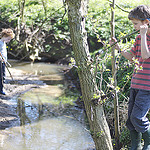
\includegraphics[width=\textwidth]{5-2_ci_prop/figures/spear}
\column{0.5\textwidth}
{\small
We can throw a spear where we saw a fish but we will probably miss. If we toss a net in that area, we have a good chance of catching the fish.
}
\column{0.25\textwidth}
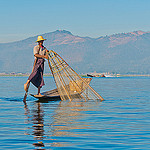
\includegraphics[width=\textwidth]{5-2_ci_prop/figures/net}
\end{columns}
$\:$ \\
\item If we report a point estimate, we probably won't hit the exact population parameter. If we report a range of plausible values we have a good shot at capturing the parameter. 

\end{itemize}

{\tiny Photos by Mark Fischer (http://www.flickr.com/photos/fischerfotos/7439791462) and Chris Penny (http://www.flickr.com/photos/clearlydived/7029109617) on Flickr.}

% spear fig: http://www.flickr.com/photos/clearlydived/7029109617/sizes/q/
% net fig: http://www.flickr.com/photos/fischerfotos/7439791462/sizes/q/

\end{frame}

%%%%%%%%%%%%%%%%%%%%%%%%%%%%%%%%%%%%

\subsection{Constructing a 95\% confidence interval}

%%%%%%%%%%%%%%%%%%%%%%%%%%%%%%%%%%%%

\begin{frame}
\frametitle{Facebook's categorization of user interests}

\dq{Most commercial websites (e.g. social media platforms, news outlets, online retailers) collect a data about their users' behaviors and use these data to deliver tageted content, recommendations, and ads. To understand whether Americans think their lives line up with how the algorithm-driven classification systems categorizes them, Pew Research asked a representative sample of 850 American Facebook users how accurately they feel the list of categories Facebook has listed for them on the page of their supposed interests actually represents them and their interests. 67\% of the respondents said that the listed categories were accurate. Estimate the true proportion of American Facebook users who think the Facebook categorizes their interests accurately.}

\ct{\webURL{https://www.pewinternet.org/2019/01/16/facebook-algorithms-and-personal-data/}}

\end{frame}

%%%%%%%%%%%%%%%%%%%%%%%%%%%%%%%%%%%%

\begin{frame}
\frametitle{Facebook's categorization of user interests}

\[ \hat{p} = 0.67 \qquad n = 850 \]

\pause

The approximate 95\% confidence interval is defined as 
\[ point~estimate \pm 1.96 \times SE \]

\pause

\vspace{-0.25cm}
\[ SE = \sqrt{\frac{p(1-p)}{n}} = \sqrt{\frac{0.67 \times 0.33}{850}} \approx 0.016 \]

\pause

\vspace{-0.25cm}
\begin{eqnarray*}
\hat{p} \pm 1.96 \times SE &=& 0.67 \pm 1.96 \times 0.016 \\
\pause
&=& (0.67 - 0.03, 0.67 + 0.03) \\
\pause
&=& (0.64, 0.70)
\end{eqnarray*}


\end{frame}

%%%%%%%%%%%%%%%%%%%%%%%%%%%%%%%%%%%

\begin{frame}
\frametitle{}

\pq{Which of the following is the correct interpretation of this confidence interval?}

We are 95\% confident that
\begin{enumerate}[(a)]
\item 64\% to 70\% of American Facebook users in this sample think Facebook categorizes their interests accurately.
\solnMult{64\% to 70\% of all American Facebook users think Facebook categorizes their interests accurately}
\item there is a 64\% to 70\% chance that a randomly chosen American Facebook user's interests are categorized accurately.
\item there is a 64\% to 70\% chance that 95\% of American Facebook users' interests are categorized accurately.
\end{enumerate}

\end{frame}

%%%%%%%%%%%%%%%%%%%%%%%%%%%%%%%%%%%

\begin{frame}
\frametitle{What does 95\% confident mean?}

\begin{itemize}

\item Suppose we took many samples and built a confidence interval from each sample using the equation $point~estimate \pm 1.96 \times SE$.

\item Then about 95\% of those intervals would contain the true population proportion ($p$). 

\end{itemize}

\end{frame}

%%%%%%%%%%%%%%%%%%%%%%%%%%%%%%%%%%%

\begin{frame}
\frametitle{Width of an interval}

\dq{If we want to be more certain that we capture the population parameter, i.e. increase our confidence level, should we use a wider interval or a smaller interval?}

\pause

\soln{A wider interval.}

$\:$ \\

\pause

\dq{Can you see any drawbacks to using a wider interval?}
\begin{center}

\includegraphics[width=0.9\textwidth]{5-2_ci_prop/figures/garfield}
\end{center}

\pause

\soln{If the interval is too wide it may not be very informative.}

{\scriptsize Image source: http://web.as.uky.edu/statistics/users/earo227/misc/garfield\_weather.gif}

\end{frame}

%%%%%%%%%%%%%%%%%%%%%%%%%%%%%%%%%%%

\subsection{Changing the confidence level}

%%%%%%%%%%%%%%%%%%%%%%%%%%%%%%%%%%%

\begin{frame}
\frametitle{Changing the confidence level}

\[ point~estimate\pm z^\star \times SE \] 

\begin{itemize}

\item In a confidence interval, $z^\star \times SE$ is called the \hl{margin of error}, and for a given sample, the margin of error changes as the confidence level changes.

\item In order to change the confidence level we need to adjust $z^\star$ in the above formula.

\item Commonly used confidence levels in practice are 90\%, 95\%, 98\%, and 99\%.

\item For a 95\% confidence interval, $z^\star = 1.96$.

\item However, using the standard normal ($z$) distribution, it is possible to find the appropriate $z^\star$ for any confidence level.

\end{itemize}

\end{frame}

%%%%%%%%%%%%%%%%%%%%%%%%%%%%%%%%%%%%

\begin{frame}

\pq{Which of the below Z scores is the appropriate $z^\star$ when calculating a 98\% confidence interval?}

\begin{multicols}{2}
\begin{enumerate}[(a)]
\item $Z = 2.05$
\item $Z = 1.96$
\solnMult{$Z = 2.33$}
\item $Z = -2.33$
\item $Z = -1.65$
\item[]
\end{enumerate}
\end{multicols}

\soln{\only<2>{
\begin{center}
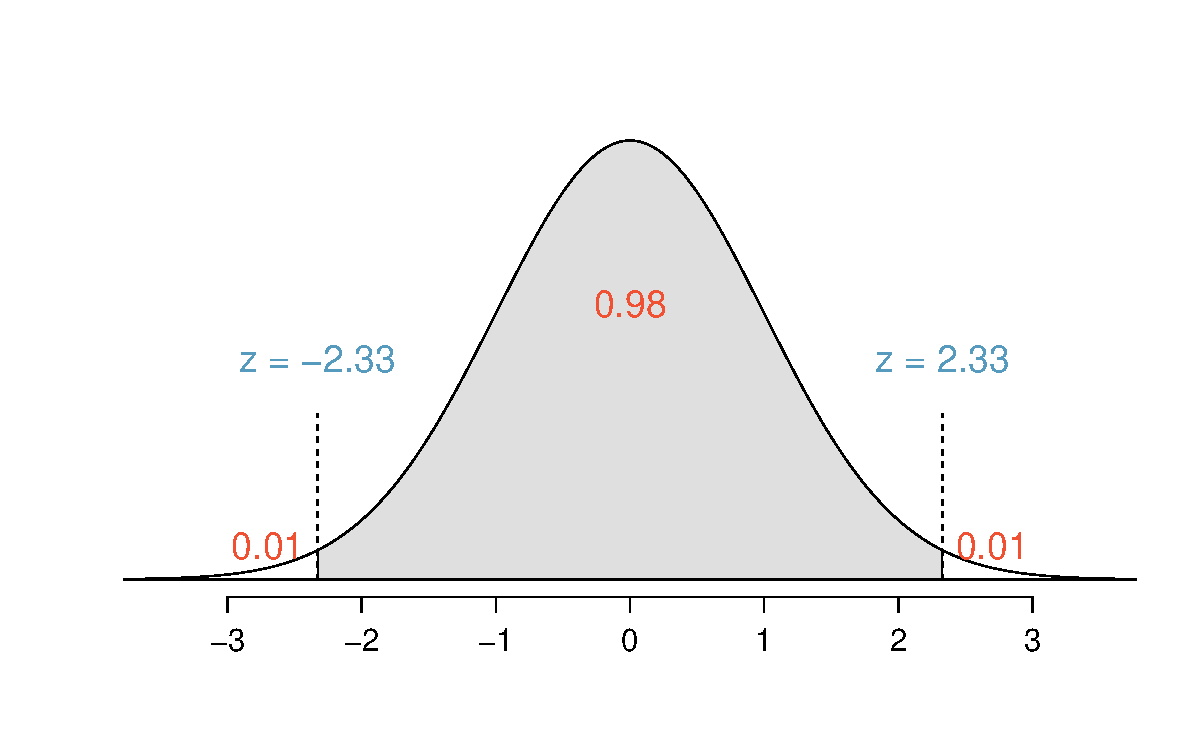
\includegraphics[width=0.7\textwidth]{5-2_ci_prop/figures/middle98/middle98}
\end{center}
}}

\end{frame}

%%%%%%%%%%%%%%%%%%%%%%%%%%%%%%%%%%%

\subsection{Interpreting confidence intervals}

%%%%%%%%%%%%%%%%%%%%%%%%%%%%%%%%%%%

\begin{frame}
\frametitle{Interpreting confidence intervals}

Confidence intervals are ...

\begin{itemize}

\item always about the population

\item are not probability statements 

\item only about population parameters, not individual observations

\item only reliable if the sample statistic they're based on is an unbiased estimator of the population parameter

\end{itemize}

\end{frame}

%%%%%%%%%%%%%%%%%%%%%%%%%%%%%%%%%%%
